\documentclass[polish,polish,a4paper]{article}
\usepackage[T1]{fontenc}
\usepackage[utf8]{inputenc}
\usepackage{babel}
\usepackage{pslatex}
\usepackage{graphicx}
\usepackage{tikz}
\usepackage{pgfplots}
\usepackage{anysize}
\usepackage{pgfgantt}
\usepackage{tabularx}
\usepackage{float}
\usepackage{latexsym,amsmath}
\marginsize{2.5cm}{2.5cm}{3cm}{3cm}


\newcommand{\name}[1]{\sffamily\bfseries\scriptsize #1}

\newcommand{\frontpage}[8]{
%% #1 - nazwa kursu
%% #2 - kierunek 
%% #3 - termin 
%% #4 - temat 
%% #5 - problem
%% #6 - data

\vspace{2cm}

\begin{tabular}{|p{0.72\textwidth}|p{0.28\textwidth}|}
\hline
\multicolumn{2}{|c|}{}\\
\multicolumn{2}{|c|}{{\LARGE #1}}\\
\multicolumn{2}{|c|}{}\\
\hline
\name{Kierunek} & \name{Termin}\\
\multicolumn{1}{|c|}{\textit{#2}} & \multicolumn{1}{|c|}{\textit{#3}} \\
\hline
\name{Temat} & \name{Problem}\\
\multicolumn{1}{|c|}{\textit{#4}} & \multicolumn{1}{|c|}{\textit{#5}} \\
\hline
\name{Prowadzący} & \name{data}\\
\multicolumn{1}{|c|}{\textit{Patryk Wlazłyń}} & \multicolumn{1}{|c|}{\textit{#6}} \\
\hline
\end{tabular}

}

\usepackage{listings}
\usepackage{xcolor} % for setting colors



% set the default code style
\lstset{ % General setup for the package
	basicstyle=\small,
	numbers=left,
	frame=tb,
	tabsize=2,
	columns=fixed,
	showstringspaces=false,
	showtabs=false,
	keepspaces,
	commentstyle=\color{red},
	keywordstyle=\color{blue}
}

\title{Sprawozdanie SPD}
\begin{document}
% #1 - nazwa kursu #2 - kierunek  #3 - termin #4 - temat #5 - problem #6 - data
\frontpage{Projektowanie Efektywnych Algorytmów}{Informatyka}{Czwartek 19:05}{Metoda przeglądu zupełnego, podzialu i ograniczeń, oraz programowanie dynamiczne.}{TSP}{\today}
\pagestyle{empty}
\newpage

\section{Opis problemu}

Problem komiwojażera (ang. travelling salesman problem, TSP) jest zagadnieniem optymalizacyjnym, polegającym na znalezieniu minimalnego cyklu Hamiltona w pełnym grafie ważonym\cite{TSPWiki:1}. Do rozwiązania problemu wymagana jest implementacja kilku struktur danych o których szerzej w dalszej częsci.
Do implementacji rozwiązania posłużył język C++, gdyż zdaniem autora pozwala on na wygodne opisywanie wysokopoziomowej abstrakcji oraz dostępne kompilatory
potrafią generować efektywny kod. Testy przeprowadzane były na systemie Ubuntu Linux 19.10 64bit z kompilatorem clang 9.0 na procesorze Intel i5-3570K (4x3.8GHz) z 8GB RAM.

\section{Struktury danych - sposób przechowywania informacji}

\subsection{Graf}

Problem komiwojażera można zdefiniować dla różnej ilości wieszchołków, dalej nazywaną wielkością problemu oraz różnych wag poszczególnych dróg łączących te wierzchołki.
Z tego względu wymaganym mechanizmem wczytywania informacji o problemie będzie plik, który zawiera wielkość grafu oraz wagi poszczególnych wierzchołków.
Wagi podawane są w postaci macierzy, w której kolejne elementy w wierszu oddzielane są znakami białymi, a same wiersze oddzielane są znakiem nowej lini.
Tak zapisane dane należy sparsować i zapisać w postaci pozwalającej na jak najprostszy oraz najszybszy sposób, ponieważ będzie ona intensywnie wykorzystywana przy rozwiązywaniu problemu.
Autor zdecydował się na przechowywanie danych w postaci kwadratowej macierzy sąsiedztwa o rozmiarze równym ilości wierzchołków.
I do jej reprezentacji została wykorzystana pojedyncza tablica typów int64\_t o rozmiarze $N^{2}$, gdzie N to rozmiar problemu.
Poniżej znajduje się definicja klasy MSTMatrix która implementuje przechowywanie macierzy sąsiedztwa.

\lstinputlisting[caption=Struktura danych MSTMatrix,language=C++]
{mst.hpp}

Jeden drobny szczegół pozostaje nie wyjaśniony - typ Edge, który klasa MSTMatrix przyjmuje jako argument przy metodzie dodawania krawędzi do grafu.
Jej implementacja jest prosta i sprowadza się do przetrzymywania informacji numeru wierzchołka źródłowego i docelowego, oraz wagi opisywanego połączenia.
Metoda MSTMatrix::add korzysta z jej pól, aby odpowiednio wypełnić informacje we własnej macierzy sąsiedztwa.
Rozwiązanie problemu będzie zwracane jako typ Path ktory jest lekkim wrapperem na klase std::vector z standardowej biblioteki.
Jego implementacja znajduje sie poniżej.

\lstinputlisting[caption=Struktura danych Path,language=C++]
{path.hpp}

Został jeszcze jeden element który wymaga krótkiego wyjaśnienia. Jest to funkcja kosztu scieżki która zwraca koszt danej scieżki na podstawie argumentu w postaci macierzy sąsiedztwa
oraz sekwencji kolejno odwiedzanych wierzchołków.

\section{Metoda rozwiązania problemu}

\subsection{Przegląd zupełny}
Metoda przeglądu zupełnego jest trywialna w koncepcji. Polega ona na przejściu przez wszystkie możliwe sposoby przebycia ścieżki w trakcie zapisując tą o dotychczasowo najniższym koszcie.
Tak, aby można było później ją odczytać. Z definicji problem wymaga odwiedzenia każdego wierzchołka dokładnie jeden raz, więc kolejnymi sposobami na przejscie przez graf są zwyczajnie
permutacje zbioru wierzchołków. Wystarczy zatem wygenerować każdą permutację i sprawdzić która jest najbardziej opłacalna. To oznacza, że wystarczy każdą permutację wysłać do funkcji
kosztu. Generowanie permutacji zostaje rozwiązane za pomocą własnej implementacji metody wykorzystanej w standardowej bibliotece pod nazwą std::next\_permutation, która jako argument 
przyjmuje posortowany kontener i generuje jego kolejną permutację w kolejności rosnącej zwracając false przy wygenerowaniu kompletnie posortowanego kontenera (stan początkowy).
Implementacja funkcji realizującej przegląd zupełny znajduje się poniżej.
\lstinputlisting[caption=Kod metody przeglądu zupełnego,language=C++]
{bt.cc}

\subsection{Metoda podziału i ograniczeń}
Tytułowa metoda polega na przechodzeniu po grafie jak po strukturze drzewiastej. W tym przypadku autor zastosował algorytm DFS (depth first search) w wersji rekurencyjnej.
Algorytm polega na wybraniu dowolnego wierzchołka i potraktowania go jako korzenia drzewa i explorowania drzewa najgłębiej jak się da i dopiero gdy spotykamy koniec drzewa wrócić do
rozważenia ścieżek wcześniej pominiętych. W trakcie przemirzeania drzewa należy sumować aktualny koszt przy każdym wykonanym kroku. I jeżeli w trakcie przechodzenia zdarzy się tak, że
aktualny koszt drogi jest w danym momencie większy od ostatniego wyniku składającego się z pełnej ścieżki, wówczas kontynuowanie przeglądu aktualnej ścieżki jest pozbawione sensu,
gdyż droga wraz z podróżowaniem nie może stać się krótsza. W takim przypadku należy wrócić do przeglądania pominiętych scieżek. Do wykonania opisanego przeszukiwania autor
zdecydował się zastosować tablicę wartości true / false aby oznaczać już odwiedzone wierzchołki.
Poniżej znajduje się rekurencyjna implementacja wspomnianaego algorytmu.
\lstinputlisting[caption=Kod metody podziału i ograniczeń,language=C++]
{dfs.cc}

\subsection{Metoda programowania dynamicznego}

Metoda programowania dynamicznego polega na takim rozwiązywaniu problemu aby po drodzę rozwiązywać podproblemy których wyniki można później wykorzystać aby przyspieszyć obliczenia
kolejnych etapów algorytmu, W tym przypadku autor skorzystał z algorytmu Helda-Karpa, który do rozwiązania poruszanego problemu korzysta z zależności problemu komiwojażera, że
\textit{Każda podścieżka scieżki bedącej optymalnym rozwiązaniem jest optymalnym rozwiązaniem}, co można zparafrazować jako właściwośc, że znajdując optymalną scieżkę dla części
węzłów mamy gwarancje, że jest ona częścią pełnej (składającej się ze wszystkich wierzchołków) optymalnej scieżki, która jest rozwiązaniem poruszanego problemu.
Wadą tego podejścia do problemu jest to, że wyniki podścieżek muszą cały czas być w pamięci na wypadek gdyby były potrzebne jako podścieżki do kolejnego rozwiązania, a mnogość
takich podrozwiązań powodują duże zużycie pamięci, które cechuje się złożonością ${2^N*N}$. Autor postanowił przechowywać wyniki podproblemów w postaci tablicy, właśnie
${2^N}$ na N. Tablica przechowuje wyniki dla każdego podzbioru problemu, który reprezentowany jest maską bitową złożoną z N bitów (dla każdego wierzchołka jeden bit), gdzie bit o wartości
true oznacza, że wierzchołek wchodzi w skład zbioru a wartość false, odwrotnie.
Dodatkowo dla każdego takiego zbioru wyznaczany jest jego wierzchołek końcowy (stąd kolejnych N możliwości zakończenia).
Poniżej znajduje się implementacja algorytmu.

\lstinputlisting[caption=kod metody programowania dynamicznego,language=c++]
{hk.cc}

Powyższy listing zawiera definicję dwóch kluczowych funkcji. Jedną z nich jest hk\_solve która jest głowną funkcją rozwiązującą rozważany problem.
hk\_solve wylicza koszty dla każdego podzbioru pełnej scieżki dla każdego jej możliwego zakończenia i zapisuje jej wynik, który wykorzystywany jest w kolejnych iteracjach algorytmu,
przy obliczaniu bardziej licznych zbiorów. Gdy funkcja ta zakończy działanie w tablicy mamy już zapisane optymalne rozwiązania dla każdego podzbioru kończoncego sie w każdym z punktów.
Kolejnym krokiem jest odtworzenie z tych danych optymalnej scieżki dla całego grafu. W tym celu wykorzystana jest funkcja hk\_find\_optimal\_path.
Wspomniana funkcja przechodzi niejako od tyłu, z gotowej scieżki dobiera najbardziej opłacalne zakończenia i wybiera je jako ostateczny wynik. Po przjściu przez wszystkie poziomy
drzewa otrzymujemy optymalną scieżkę którą możemy zwrócić jako wynik.

\section{Eksperymenty obliczeniowe}
Czas wykonywanych operacji był mierzony na systemie opisanym w wprowadzeniu.
Do pomiaru czasu wykorzystano standardową bibliotekę języka C++, biblioteke std::chrono.
Pomiar czasu wykonywany był w nanosekundach. Każdy pomiar wykonywany był 50 razy i ostatecznym wynikiem była średnia czasu z wszystkich prób.
Dodatkowo przed dokonywaniem takiego pomiaru uruchamiano 10 razy przebieg mierzonego kawałka kodu bez mierzenia jego czasu po to aby wytrenować układy przewidywania odwoływań do pamięci,
tj. branch prediction, cache prefetching.
Poniżej znajduje się kod realizujący mierzenie czasu.

\lstinputlisting[caption=kod metody programowania dynamicznego,language=c++]
{timeutils.hpp}

\pagebreak
\begin{center}
\begin{tabularx}{0.5\textwidth} { 
	| >{\centering\arraybackslash}X 
	| >{\centering\arraybackslash}X | }
	\hline
	\multicolumn{2}{|c|}{Metoda przeglądu zupełnego} \\
	\hline
	Wielkość problemu & Czas wykonania (ns) \\
	\hline
	2 & 328 \\
	\hline
	3 & 691 \\
	\hline
	4 & 3026 \\
	\hline
	5 & 17928 \\
	\hline
	6 & 80026 \\
	\hline
	7 & 442466 \\
	\hline
	8 & 3953679 \\
	\hline
	9 & 39880219 \\
	\hline
	10 & 442507917 \\
	\hline
	11 & 5353492295 \\
	\hline
\end{tabularx}

\bigskip

\begin{tabularx}{0.5\textwidth} { 
	| >{\centering\arraybackslash}X 
	| >{\centering\arraybackslash}X | }
	\hline
	\multicolumn{2}{|c|}{Metoda przeszukiwanuia w głąb} \\
	\hline
	Wielkość problemu & Czas wykonania (ns) \\
	\hline
	2 & 225 \\
	\hline
	3 & 699 \\
	\hline
	4 & 1469 \\
	\hline
	5 & 6033 \\
	\hline
	6 & 21570 \\
	\hline
	7 & 84161 \\
	\hline
	8 & 179542 \\
	\hline
	9 & 730287 \\
	\hline
	10 & 2420364 \\
	\hline
	11 & 5190784 \\
	\hline
	12 & 92879242 \\
	\hline
	13 & 546526194 \\
	\hline
	14 & 103633643 \\
	\hline
\end{tabularx}

\bigskip

\begin{tabularx}{0.5\textwidth} { 
	| >{\centering\arraybackslash}X 
	| >{\centering\arraybackslash}X | }
	\hline
	\multicolumn{2}{|c|}{Metoda dynamiczna Helda-Karpa} \\
	\hline
	Wielkość problemu & Czas wykonania (ns) \\
	\hline
	2 & 205 \\
	\hline
	3 & 854 \\
	\hline
	4 & 2780 \\
	\hline
	5 & 3429 \\
	\hline
	6 & 8669 \\
	\hline
	7 & 22836 \\
	\hline
	8 & 51377 \\
	\hline
	9 & 117697 \\
	\hline
	10 & 288131 \\
	\hline
	11 & 651784 \\
	\hline
	12 & 1481028 \\
	\hline
	13 & 3447888 \\
	\hline
	14 & 7751161 \\
	\hline
	15 & 17600188 \\
	\hline
	16 & 41210060 \\
	\hline
	17 & 94666222 \\
	\hline
	18 & 230991845 \\
	\hline
\end{tabularx}
\end{center}

\newpage

\begin{figure}[H]
\begin{center}
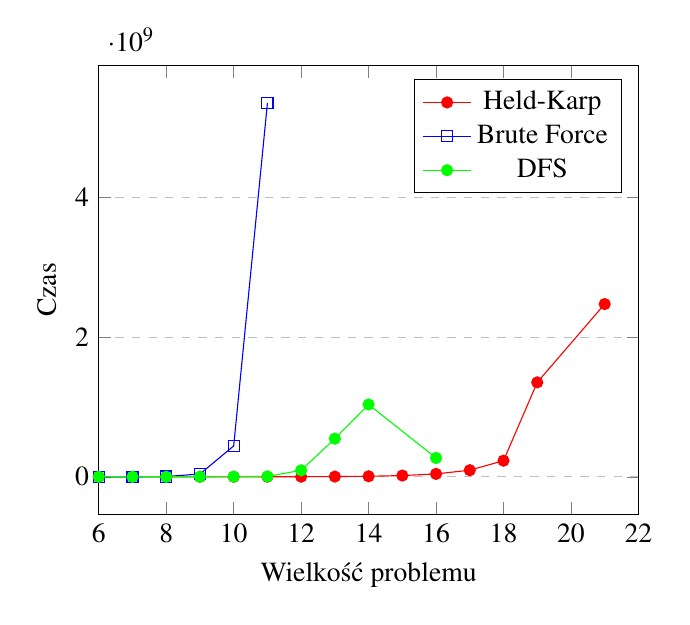
\begin{tikzpicture}
	\begin{axis}[
		xlabel=Wielkość problemu,
		ylabel=Czas,
		ymajorgrids=true,grid style=dashed,
		legend pos=north east,
		xmin=6,
		xmax=22
	]
	\addplot[color=red,mark=*]
	coordinates {
		(2,205)
		(3,854)
		(4,2780)
		(5,3429)
		(6,8669)
		(7,22836)
		(8,51377)
		(9,117697)
		(10,288131)
		(11,651784)
		(12,1481028)
		(13,3447888)
		(14,7751161)
		(15,17600188)
		(16,41210060)
		(17,94666222)
		(18,230991845)
		(19,1353198041)
		(21,2475404238)
	};

	\addplot[color=blue,mark=square]
	coordinates {
		(2,328)
		(3,691)
		(4,3026)
		(5,17928)
		(6,80026)
		(7,442466)
		(8,3953679)
		(9,39880219)
		(10,442507917)
		(11,5353492295)
	};

	\addplot[color=green,mark=*]
	coordinates {
		(2,225)
		(3,699)
		(4,1469)
		(5,6033)
		(6,21570)
		(7,84161)
		(8,179542)
		(9,730287)
		(10,2420364)
		(11,5190784)
		(12,92879242)
		(13,546526194)
		(14,1036336434)
		(16, 270100653)
	};

\legend{Held-Karp, Brute Force, DFS}

\end{axis}
\end{tikzpicture}
\caption{Czas wykonywania się algorytmów w zależności od wielkości problemu}
\end{center}

\begin{center}
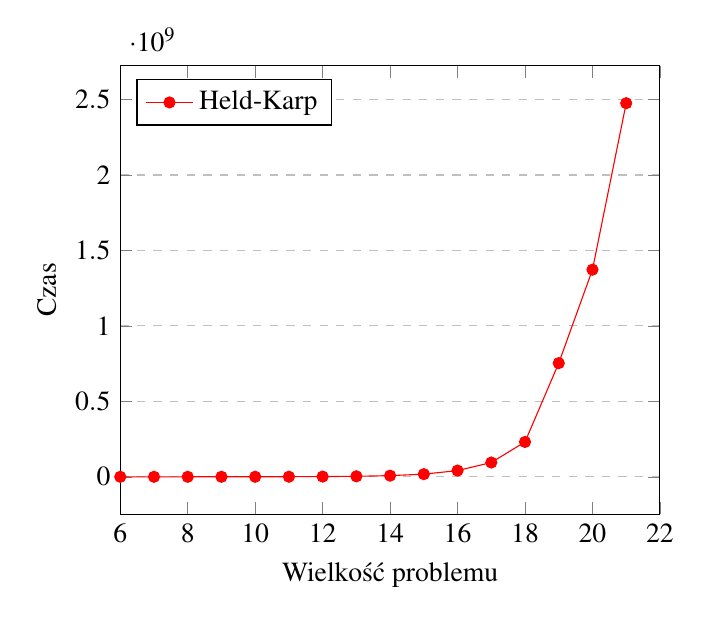
\begin{tikzpicture}
	\begin{axis}[
		xlabel=Wielkość problemu,
		ylabel=Czas,
		ymajorgrids=true,grid style=dashed,
		legend pos=north west,
		xmin=6,
		xmax=22
	]
	\addplot[color=red,mark=*]
	coordinates {
		(2,205)
		(3,854)
		(4,2780)
		(5,3429)
		(6,8669)
		(7,22836)
		(8,51377)
		(9,117697)
		(10,288131)
		(11,651784)
		(12,1481028)
		(13,3447888)
		(14,7751161)
		(15,17600188)
		(16,41210060)
		(17,94666222)
		(18,230991845)
		(19,753198041)
		(20,1372398544)
		(21,2475404238)
	};

\legend{Held-Karp}

\end{axis}
\end{tikzpicture}
\caption{Czas wykonywania się algorytmów w zależności od wielkości problemu}
\end{center}
\end{figure}

\newpage

\section{Wnioski}
\hspace{\parindent}
\par
Algorytm przeglądu zupełnego okazał się być (jak oczekiwano) najmniej efektywnym sposobem rozwiązania problemu. Biorąc pod uwage implementacje generowania permutacji nie jest też
metoda najprostszą do zaimplementowania z tych prezentowanych. Algorytm polega na porównaniu każdej możliwej scieżki wiec jego złożoność to n!, gdyż jest to równoważne z wygenerowaniem
każdej możliwej permutacji zbioru wierzchołków. Metoda jest zwyczajnie nie praktyczna. \\

\par
Algorytm przeglądania drzewa w głąb okazał się być najprostszy do zaimplementowania. Dla każdego nie odwiedzonego jeszcze sąsiada wywołujemy rekurencyjnie procedure.
Dzięki wprowadzeniu dodatkowego sprawdzania aktualnego kosztu drogi możemy wcześniej stwierdzić już na danym etapie, że dane rozwiązanie nie może dać lepszego rezultatu niż najlepszy
dotychas znany, wówczas możemy "odciąć" to rozwiązanie i przejść do sąsiedniego rozgałęzienia. Ta metoda jednak nie daje dużo lepszych rezultatów czasowych. Jest co prawda nieco szybsza,
a tempo wzrostu w praktyce okazuje się dużo bardziej "gładkie", ale nadal nie daje zadowalających rezultatów. Dodatkowo dla różnych danych dostajemy kompletnie różne złożoności, które
wydają się nie być opisywalne żadną uniwersalną złożonością. Wynika to z tego, że sytuacje w których faktycznie "odcinamy" nie opłacalne rozgałęzienia mogą pojawiać się bardzo późno
w trakcie przeszukiwania co prowadzi do tego, że i tak algorytm bedzie musiał przejść przez większość drzewa. \\

\par
Algorytm programowania dynamicznego Helda-Karpa cechuje sie złożonością czasową O($2^nn^2$).
Jego wadą jest jednak duża złożoność pamięciowa ze względu na alokacje dużej tablicy do zapisywania wyników dla podzbiorów wierzchołków, która wynosi O($2^nn$).
Właśnie przez swoją złożoność pamięciową oraz (nadal) długi czas wykonania algorytm nie przydaje sie w praktycznych rozwiązaniach.

\bibliographystyle{abbrv}
\bibliography{ref}
\end{document}

